\textit{Определение} \textit{Маргинальной} называют вероятность $P(A)$ события $A$ 
наступить в независимости от наступления прочих. 

Маргинальное распределение $P(X) = \int P(X, \theta) d\theta$ позволяет
подбирать оптимальные конфигурации байесовых сетей под задачу и обновлять параметры
распределений согласно наблюдениям $e$: $P(Y| E=e) = \frac{P(Y,E=e)}{P(E=e)}$.

В общем случае расчет маргинального распределения является NP-сложной задачей, 
тем не менее существуют эффективные алгоритмы аппроксимации.

\begin{figure}[h]
    \centering
    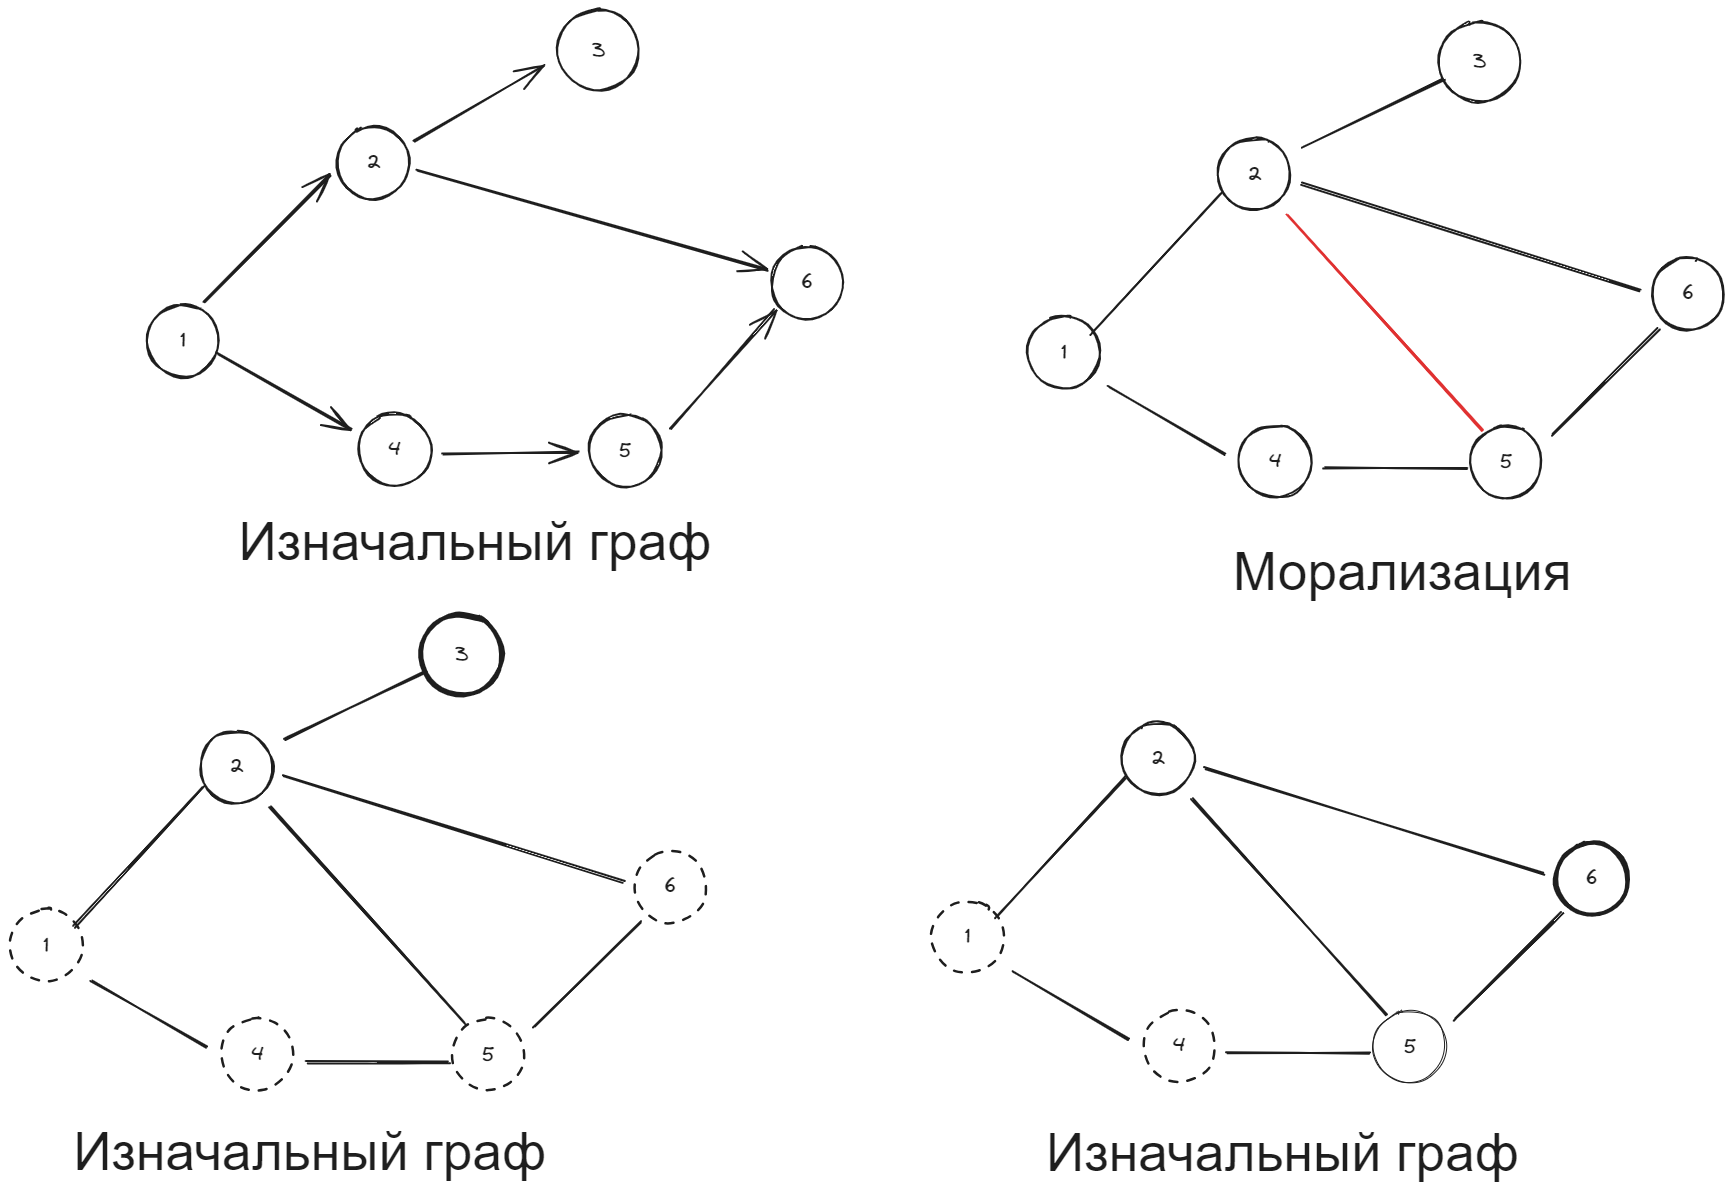
\includegraphics[width=0.5\textwidth]{assets/math/discrete/elimination.excalidraw.png}
    \caption{Расчет распространения доверия от узлов}
    \label{elimination}
\end{figure}

Одним из базовых алгоритмов является алгоритм исключения переменных (\textit{англ}. Variable Elimination).
В такой постановке изначально задает порядок обхода $O$ \ref{elimination}. В последствии для каждой переменной
из обхода $X_i$ выполняется:\begin{enumerate}
    \item произведение всех факторов $\phi_i$ содержащих $X_i$
    \item маргинализация по $X_I$ для получения нового фактора $\tau$
    \item замена факторов $\phi_i$, содержащих $X_i$, на $\tau$ в итоговом статистическом произведении 
\end{enumerate} 

На практике применяется обобщение алгоритма исключения перменных. Формирование маргинализованного фактора
$\tau$ выполняется.

\texit{Определение} \texbf{Алгоритмы передачи сообщений} заключаются в 
Передача сообщения от переменной к фактору

В случае отсустствия циклов сообщения распространяются от узла к узлу


\begin{figure}[h]
    \centering
    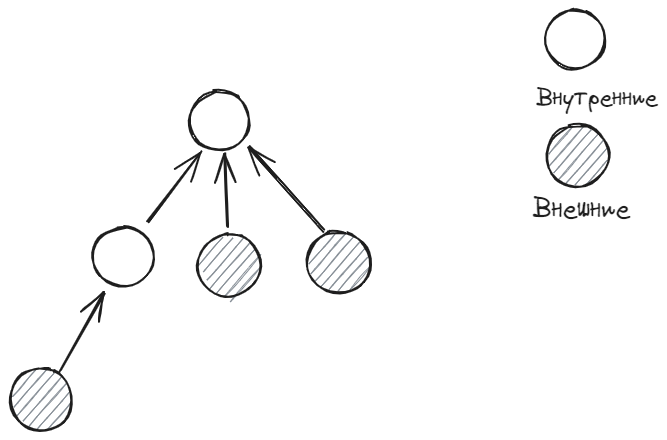
\includegraphics[width=0.5\textwidth]{assets/math/discrete/belief_propogation.excalidraw.png}
    \caption{Расчет распространения доверия от узлов}
    \label{discr_vs_gen}
\end{figure}

Формально передача сообщений записывается как алгоритм:
\begin{equation}
    \begin{aligned}
        &m_{f_j \rightarrow x_i} = \sum_{X_j \backslash x_i} f_j(X_j) \prod_{k\in N(j) \ i} m_{x_k \rightarrow f_j}\\
        &m_{x_i \rightarrow f_j} = \prod_{s \in N(i) \backslash j} m_{f_s \rightarrow x_i}
    \end{aligned}
\end{equation}
Обновление вероятностных распределений выполняется путем произведения всех входящих сообщений 
\begin{equation}
    b_i(x_i) = \prod_{s\in N(i)} m_{f_s \rightarrow x_i}
\end{equation}

\texit{Теорема}\cite{yedidia2000generalized} Алгоритм передачи сообщений сходится к истинному распределению
в $KL$ дивергенции $\limKL(q,p) \rightarrow 0$. 
\texit{Доказательство}

Запишем $\text{KL}$ дивергенцию между апостериорным $p$ и априорным распределением $q$:
\begin{equation}
    \texit{KL}(q \parallel p)= \sum_{X} q(X) \log \frac{q(X)}{p(X)}
\end{equation}

Используем факторизацию $p(X)= \frac{1}{Z} \prod_a \exp^{-E(X_a)}$:
\begin{equation}
    \texit{KL}(q \parallel p)= \sum_{X} q(X) \log q(X) - \mathbb{E}_q \log p(X) = - H_q(X) - \sum_a \matbb{E}_q \log f_a(X_a) +log(Z)
\end{equation}

С$F(p,q) = - H_q(X) - \sum(a) \matbb{E}_q \log f_a(X_a $

Для случая дерева свободная энергия запишется как:
\begin{equation}
    q(X) = \prod_i b_i(x_i)^{1-d_i} \prod_a b_a(X_a), где
\end{equation}
первый член произведения задает произведения вероятности переменных, а второй произведения вероятности клик. Энтропия такого
распределения запишется как:
\begin{equation}
    H_{\tree} = - \sum_i (1-d_i) \sum_{x_i} b_i(x_i) \log b_i (x_i) - \sum_a \sum_X_A b_a(X_a) \log b_a(X_A)
\end{equation}

Тогда свободная энергия древа запишется как:
\begin{equation}
    F_{\text{tree}} = -\sum_i (d_i -1) \sum_{x_i} b_i(x_I) \log b_i(x_i) + \sum_a \sum_X_A b_a(X_a) \log \frac{b_a(X_A)}{f_a(X_a)}
\end{equation}
Лангражиан выражения c условиями нормализации $b_i = \sum_{X_a \backslash i} b_a(X_a)$ и $\sum_i b_i(x_i) =1$ запишется ка:
\begin{equation}
    L = F_{\text{\Bethe}} + \sum_i \gamma_i \left{1- \sum_{x_i} b_i(x_i)\right} + \sum)a
\end{equation}

Тогда :
\begin{equation}
    \frac{\partial L}{\partial b_i(x_i)} = 0 \Rightarrow b_i \sim \prod m_{x_i \rightarrow f_a} (x_i)
\end{equation}

\begin{equation}
    \frac{\partial L}{\partial b_i(x_i)} = 0 
\end{equation}

Тогда из условия получаем

$\blacksquare$

Наиболее численно эффективным является модели гауссового распостранения доверия. В таких постановках 
энергия клики $E(X_C)$ записывается через квадратичную форму
\begin{equation}
    P(X_C) \sim \exp(-\frac{1}{2}X^T \lambda X + \eta^T X),
\end{equation}
где параметры $\lambda \in \mathbb{R}^{\deg{C} \times deg{C}}$ и $\eta \in \mathbb{R}^{deg{C}}$. 